\section{Straight-Line Program}
\label{slpsec}
% Algorithmics on SLP-Compressed Strings: A Survey
% Practical Random Access to SLP-Compressed Texts
% PHONI: Streamed Matching Statistics with Multi-Genome References
% Indexing Highly Repetitive String Collections
Nel contesto \textit{bioinformatico} una delle principali problematiche è la
gestione di testi molto estesi. Pensiamo, ad esempio, al caso umano. Il primo
cromosoma, il più lungo tra i cromosomi umani, conta circa $247.249.719$
\textit{bps} (paia di basi), nonostante, è bene segnalare, l'uomo
non sia affatto l'essere vivente con il genoma più esteso. Fatta questa breve
premessa è facile comprendere l'importanza degli algoritmi e delle strutture
dati atte alla compressione di testi.\\
Per questa tesi si è provveduto all'uso di uno di tali algoritmi di
compressione, ovvero i \textbf{Straight-line programs (\textit{SLPs})}. Parlando
in termini generici un \textit{SLP} è una \textbf{grammatica context-free} che
genera una e una sola parola \cite{slpsurvey}. Si parla, a causa di ciò, di
\textbf{grammar-based compression}.
\begin{definizione}
  Sia dato un alfabeto finito $\Sigma$ per i simboli terminali. Sia data una
  stringa $s=a_1,a_2,\ldots, a_n\in\Sigma^{*}$, lunga $n$ e costruita
  sull'alfabeto $\Sigma$. Si ha quindi che $a_i\in\Sigma$, $\forall i \mbox{
    t.c. }1\leq i\leq n$, denotando con $alph(s)=\{a_1,a_2,\ldots
  a_n\}$ l'insieme dei simboli della stringa $s$.\\
  Un \textbf{SLP} sull'alfabeto $\Sigma$ è una grammatica context-free
  $\mathcal{A}$: 
  \[\mathcal{A}=\left(\mathcal{V}, \Sigma, \mathcal{S}, \mathcal{P}\right)\]
  dove:
  \begin{itemize}
    \item $\mathcal{V}$ è l'insieme dei simboli non terminali
    \item $\Sigma$ è l'insieme dei simboli terminali
    \item $\mathcal{S}\in \mathcal{V}$ è il simbolo iniziale non terminale
    \item $\mathcal{P}$ è l'insieme delle produzioni, avendo che:
    \[\mathcal{P}\subseteq \mathcal{V}\times\left(\mathcal{V}\cup
        \Sigma\right)^{*}\] 
  \end{itemize}
  Tale grammatica, per essere un \textit{SLP}, deve soddisfare due proprietà:
  \begin{enumerate}
    \item si ha una e una sola produzione $(A,\alpha)\in \mathcal{P}$, $\forall
    A\in \mathcal{V}$ con $\alpha\in \left(\mathcal{V}\cup\Sigma\right)^{*}$ (si
    noti che la produzione $(A,\alpha)$ può anche essere indicata con
    $A\to\alpha$) 
    \item la relazione $\{(A,B)\,|\,\,(A,\alpha)\in\mathcal{P},\,\,B\in
    alph(\alpha)\}$ è aciclica
  \end{enumerate}
  Si ha quindi che la grandezza dell'SLP è calcolabile come:
  \[|\mathcal{A}| = \sum_{(A,\alpha)\in\mathcal{P}}|\alpha|\]
\end{definizione}
Si ha quindi che il linguaggio generato da un \textit{SLP}, $\mathcal{A}$,
consiste in una singola parola, denotata da $eval{\mathcal{A}}$. \\
A partire dall'\textit{SLP} $\mathcal{A}$ si genera quindi un \textbf{albero
  di derivazione}, che nel dettaglio è un \textit{albero radicato e ordinato},
dove la \textit{radice} è etichettata con $\mathcal{S}$, ogni \textit{nodo
  interno} è etichettato con un simbolo di $\mathcal{V}\cup\Sigma$ e ogni foglia
è etichettata con un simbolo di $\Sigma$.\\
Si vede quindi un esempio chiarificatore \cite{slpgagie}.
\begin{esempio}
  \label{ese:slpgagie}
  Si prenda la seguente stringa:
  \[s=\mbox{GATTAGATACAT}\,\$\mbox{GATTACATAGAT}\]
  Si potrebbe produrre il seguente \emph{SLP}:
  \[\mbox{S}\to \mbox{ZWAY}\,\$\mbox{ZYAW}\]
  \[\mbox{Z}\to \mbox{WX}\]
  \[\mbox{Y}\to \mbox{CV}\]
  \[\mbox{X}\to \mbox{TA}\]
  \[\mbox{W}\to \mbox{GV}\]
  \[\mbox{V}\to \mbox{AT}\]
  Al quale corrisponde il seguente \emph{albero di derivazione}, dove il simbolo
  iniziale non terminante, ovvero la radice, è indicata con un cerchio giallo, i
  simboli non terminanti, ovvero i nodi interni, sono indicati dai cerchi blu
  mentre i simboli terminanti, ovvero le foglie, sono indicati dai quadrati
  verdi:
  \begin{figure}[H]
    \centering
    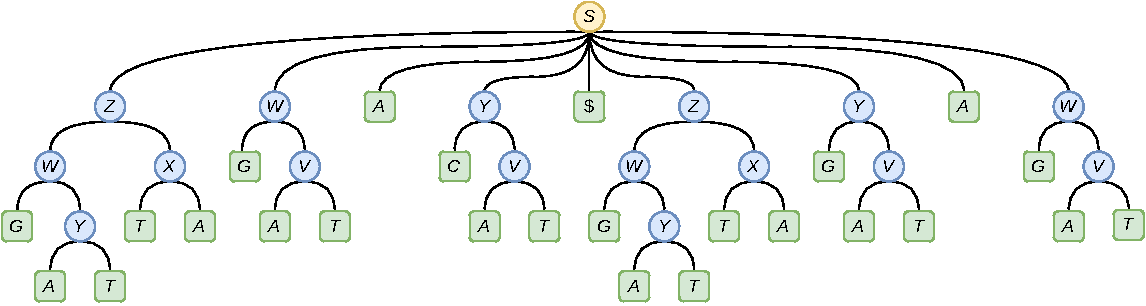
\includegraphics[width=\textwidth]{img/slpgagie.pdf}
  \end{figure}
\end{esempio}
Nel 2020, Gagie et al. \cite{slpgagie}, a cui si rimanda per approfondimenti,
proposero una variante degli \textit{SLPs} che garantisse miglioramenti
prestazionali per il \textit{random access} alla grammatica stessa. Sfruttando,
ad esempio, i \textit{bit vector sparsi} si è quindi potuto garantire
\textit{random access} su un testo $T$, tale che $|T|=n$, compresso tramite
\textit{SLP}, in tempo:
\[\mathcal{O}(\log n)\]
\textbf{VERIFICARE BENE COSA SIA $n$}.\\
L'uso di tale variante degli \textit{SLP} è stato cruciale, come si vedrà più
avanti in questa tesi, per la costruzione della versione run-length encoded sia
della \textbf{Burrows-Wheeler Transform (\textit{BWT})} che della
\textbf{Positional Burrows-Wheeler Transform (\textit{PBWT})}.
\subsection{Longest Common Extension}
Oltre a permettere un veloce \textit{random access} alla testo compresso, la
variante degli \textit{SLPs} proposta da Gagie et al. permette di effettuare
un'altra operazione in modo ``veloce'': le \textbf{Longest Common Extension
  (\textit{LCE}) queries}.
\begin{definizione}
  Dato un testo $T$, tale che $|T|=n$, il risultato della \textbf{LCE query} tra
  due posizioni $i$ e $j$, tali che $0\leq i,j<n$, corrisponde al più lungo
  prefisso comune tra le sotto-stringhe che hanno come indice di partenza $i$ e
  $j$, avendo quindi il più lungo prefisso comune tra $T[i:n-1]$ e $T[j:n-1]$.
\end{definizione}
Sfruttando l'\textit{SLP} del testo $T$ è quindi possibile effettuare due
\textit{random access} al testo compresso, in $i$ e $j$, per poi ``risalire''
l'albero al fine di computare il prefisso comune tra $T[i:n-1]$ e
$T[j:n-1]$. Quindi il calcolo di una \textit{LCE query} di lunghezza $l$ è
effettuabile in tempo:
\[\mathcal{O}\left(1+\frac{l}{\log n}\right)\]
\textbf{VERIFICARE BENE COSA SIA $n$}.